\setchapterstyle{kao}
\setchapterpreamble[u]{\margintoc}

\setcounter{chapter}{9}

%%% For material score
\newcommand{\outerradius}{1cm}
\newcommand{\innerradius}{.75cm}
\newcommand{\barlength}{2cm}
\newcommand{\barheight}{1.5mm}
\newcommand{\barypos}[1]{- \outerradius + #1 * \outerradius / 2 - \outerradius / 4 - \barheight / 2}

\newcommand{\materialscore}[6]{
\begin{tikzpicture}

    \fill[gr20] (0,0) circle (\outerradius);
    \fill[gr50] (0,0) -- (0, \outerradius)
      arc (90:90-36*#2:\outerradius) -- (0,0);
    \fill[white] (0,0) circle (\innerradius);

     \node[gr70] at (\outerradius + 5mm, \barypos{4} + \barheight / 2) {\faIcon{magnet}};
     \fill[gr20] (\outerradius + 9mm, \barypos{4}) rectangle ++(\barlength, \barheight);
     \fill[gr50] (\outerradius + 9mm, \barypos{4}) rectangle ++(\barlength * 0.1 * #3, \barheight);

    \node[gr70] at (\outerradius + 5mm, \barypos{3} + \barheight / 2) {\faIcon{fire}};
    \fill[gr20] (\outerradius + 9mm, \barypos{3}) rectangle ++(\barlength, \barheight);
    \fill[gr50] (\outerradius + 9mm, \barypos{3}) rectangle ++(\barlength * 0.1 * #4, \barheight);

    \node[gr70] at (\outerradius + 5mm, \barypos{2} + \barheight / 2) {\faIcon{euro-sign}};
    \fill[gr20] (\outerradius + 9mm, \barypos{2}) rectangle ++(\barlength, \barheight);
    \fill[gr50] (\outerradius + 9mm, \barypos{2}) rectangle ++(\barlength * 0.1 * #5, \barheight);

    \node[gr70] at (\outerradius + 5mm, \barypos{1} + \barheight / 2) {\faIcon{eye}};
    \fill[gr20] (\outerradius + 9mm, \barypos{1}) rectangle ++(\barlength, \barheight);
    \fill[gr50] (\outerradius + 9mm, \barypos{1}) rectangle ++(\barlength * 0.1 * #6, \barheight);

    \foreach \l in {1,...,4}{
      \foreach \p in {1,...,9}{
        \draw[gr20, ultra thick] (\outerradius + 9mm + \barlength / 10 * \p, \barypos{\l}) -- ++(0, \barheight);
      }
    }

    \foreach \a in {0,36,72,...,360}{
      \draw[gr20, ultra thick] (\a+18:\innerradius) -- (\a+18:\outerradius);
    }

    \node at (\outerradius / 2 + \barlength / 2, \outerradius * 1.25){\large{\textbf{#1}}};
\end{tikzpicture}}

\chapter{Casing}

% Since the tesla coil is intended as a consumer product, the casing plays an important role for its appearance. But apart from optics, there are a lot of safety hazards, which the casing has to account for. Most notably is the very real fire risk, which goes along playing with open plasma.

% Another point to note is, that the casing was build with modularity in mind. This enables to repair 
It might seem like the casing is not very significant, even though the design and function of all kinds of device's exteriors is crucial. The simplest of casings often have multiple design stages and variations with different advantages. When designing something as complex and difficult as a tesla coil, the casing is even more rigorous to construct. 


\section{Concept design}
\label{sec:concept-design}

There are four main parts that are essential to consider while constructing the tesla coil - the primary coil, the secondary coil, the \gls{pcb}, and the top electrode. Those can be placed in any way possible, but there is a reasonable standard practice for their placement, especially for the coils and the top electrode. 

\begin{figure}
    \centering
    %\missingfigure
    %\includegraphics{}
    \caption{Concept design}
    \label{BD-envision}
\end{figure}

As seen above, the secondary coil is perpendicular, and the primary coil is angled at 30°\sidenote{The primary coil design choices have already been explained in the previous part at the end of \ref{sec:designing-the-primary}} to the horizontal. This is the easiest way to calculate and most practical way to design the secondary. The placement for the top electrode seems very obvious, but there is an explanation. If the arching point of the electrode is placed further away from the secondary, the behavior of the coils will become less predictable the more distance is between them. So the most practical placement is in the middle and a few centimeters above the secondary coil.

Technically the \gls{pcb} can be placed anywhere\sidenote{There should be a reasonable distance between the PCB and the coils to ensure that the electrical field does not interfere with the circuitry.} as long as it can be connected to the coils. However, to make transportation the easiest, the casing for the \gls{pcb} should be right beneath the coils. This way, everything needed stays in one place. 

\section{Materials}

Deciding which materials to use is also a tedious task because there are a lot of details and possibilities that have to be considered when designing a tesla coil. Many factors determine the best working material, most affecting the coils directly and therefore being unsuitable, but others are scrapped because of their low availability or costly construction.

\subsection{Metals}
\label{subsec:materials-metals}

Metal is a popular choice for building high-grade casings because of its low price and good machinability. However, metals are rather unsuitable for a tesla coil, mainly because of their electrical conductivity, which would pose an unnecessary safety risk to the user when touched. On one side, because some internal connection error could be lethal in the worst case, but also because if not properly grounded, static electricity could build up in the casing and shock everyone touching it. Another critical factor is that metals have very high permeability, weakening any magnetic field. This would not be a big problem for the \gls{pcb} enclosure but would certainly cause issues when used around the primary or secondary coil.

\subsection{Woods}

One material that is not often used for casings, especially for commercial products, is wood, mainly because it is more expensive and harder to work with than metal. This tesla coil is not like any device, but wood is still not a good option, mainly because the top electrode emits a high-temperature spark which could inflame the wooden casing. Making the casing for only the board wooden would not work either because if the capacitance of the secondary coil changes, the driver operates outside of its ideal conditions and dissipates a lot of energy as heat, potentially inflaming the wood.

\subsection{Glass}

Glass is an electrical insulator, so it would not interfere with the magnetic field, has very high-temperature resistance, and has a polished look. It also comes in various opacities, and surface finishes making the casing very customizable. The main disadvantage of glass is its high production costs. Due to the tesla coil not being commercially produced, this kind of casing is unsustainable.

\subsection{Plastics}

\glsunset{pvcp}\glsunset{pmma}\glsunset{pvcu}\glsunset{ptfe}
The only remaining option for the type of casings material would be plastic. However, plastic is not plastic. The two types of plastic with the highest availability, in this case, would be \gls{pvcp} and \gls{pmma}\sidenote{also commercially known as acrylic glass or plexiglass}. There is also \gls{pvcu}, but given that it is harder to process and also less available, \gls{pvcp} is preferred. \gls{pvcp} would be a lot better than \gls{pmma} when it comes to cost and availability, but it cannot provide the suitable characteristics for the tesla coil. One problem with \gls{pvcp} is its water absorption because due to water's diamagnetic properties, it heats up in an oscillating magnetic field, i.e., it is wasting energy. \gls{pvcp}s water absorption over 24 hours lies at a maximum of 1\% of its total weight. \gls{pmma}, in comparison, has an absorption of 0.4\% at max. On the other hand, \gls{pvcu} has an even more ideal water absorption at 0.1\%. The casing should not be out of \gls{pvcp} or \gls{pvcu} because of its poor temperature resistance, which starts to deform at around 60°C, while \gls{pmma} only starts at about 100°C. \gls{pmma} is not ideal in any way, but due to its easy availability and better properties, it was chosen for the casing. 

The ideal plastic would be \gls{ptfe}\sidenote{also commercially known as Teflon}, which has a maximum of 0.01\%, a tenth better than \gls{pvcu}. The temperature resistance is also better than \gls{pmma} because it can be used at a working temperature of 280°C\sidecite{blue-bible}. \gls{ptfe} was not used as a casing because it was unavailable, but it might be considered in a future build.  

\todo{Welche veraussetzung die materialien haben müssen und warum gewisse nicht in frage kommen. Berechnungen auch Permeabilität \& Permittivität
https://omnexus.specialchem.com/polymer-properties/properties/water-absorption-24-hours einbinden}

\subsection{Conclusion}

In figure \ref{fig:material-score}, all previously discussed materials are given a subjective score from 1 to 10 in the four most important categories. The score in the circle is then determined by the average points of these categories, quickly visualizing which material is best suited for the tesla coil. Both \gls{ptfe} and \gls{pmma} have the same total score, but as already mentioned above, \gls{ptfe} wasn't used because of the low availability.  

\begin{figure}[h!]
    \centering
    \begin{tabular}{cc}
      \materialscore{Metal}{4}{1}{8}{6}{3} & \materialscore{Wood}{5}{6}{2}{7}{6} \\
      \materialscore{Glass}{7}{9}{9}{1}{10} & \materialscore{PMMA}{8}{8}{6}{9}{7} \\
      \materialscore{PVC-U}{7}{9}{6}{9}{5} & \materialscore{PTFE}{8}{10}{7}{8}{6} \\
      \multicolumn{2}{l}{
      \begin{tabular}{cl}
        \\
        {\color{gr70}\faIcon{magnet}} &  Magnetic and Electrical Properties \\
        {\color{gr70}\faIcon{fire}} &  Temperature resistance \\
        {\color{gr70}\faIcon{euro-sign}} &  Machinability and cost \\
        {\color{gr70}\faIcon{eye}} &  Optics
      \end{tabular}}
    \end{tabular}
    \caption{Bottom text}
    \label{fig:material-score}
\end{figure}



\section{Structure for the Coils}

As mentioned in section \ref{sec:concept-design}, both coils have a fixed position and shape, but to ensure this, the casing has to be built based on them. The secondary is easy to support, but the primary has a unique shape that has to be kept in form. 

\subsection{Primary Coil}

The primary coil's holding structure consists of six supports arranged in a hexagonal way. Every support is a triangular-shaped slope with an angle of 30°, on top of which the primary coil rests. In order to keep the primary coil in place, small half-circles have been cut out for every turn. However, to keep the coil's shape, the ten slots on each support have to be shifted up by one-sixth of the distance between each other.

\begin{figure}[h!]
    \centering
    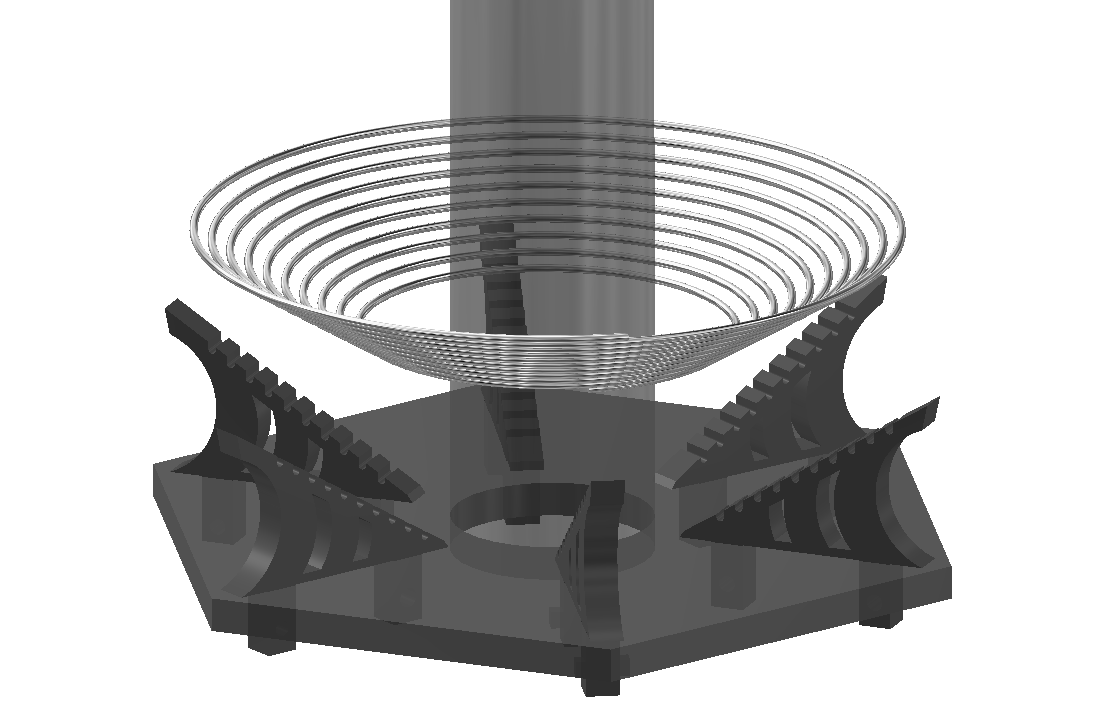
\includegraphics[width=1\textwidth]{kassandra/resources/endeMeinerHoffnung.png}
    \caption{3D view of the primary supports}
    \label{fig:primary-supports}
\end{figure}

To avoid gluing the supports to the base plate, a bolt was used to keep it in place, as shown in figure \ref{fig:stayer}. This mechanism was mainly designed for testing purposes as it is easier to assemble and disassemble. In a possible future version or commercial release, it would be safer if the supports were glued on. Also, as shown, the supports have a unique design. This was mostly done to make them look elegant and not stand out too much. That makes them lighter, but given that the supports are just a tiny fraction of the tesla coil's weight, it does not make much difference.

\begin{figure}[h!]
    \begin{subfigure}{0.5\textwidth}
        \centering
        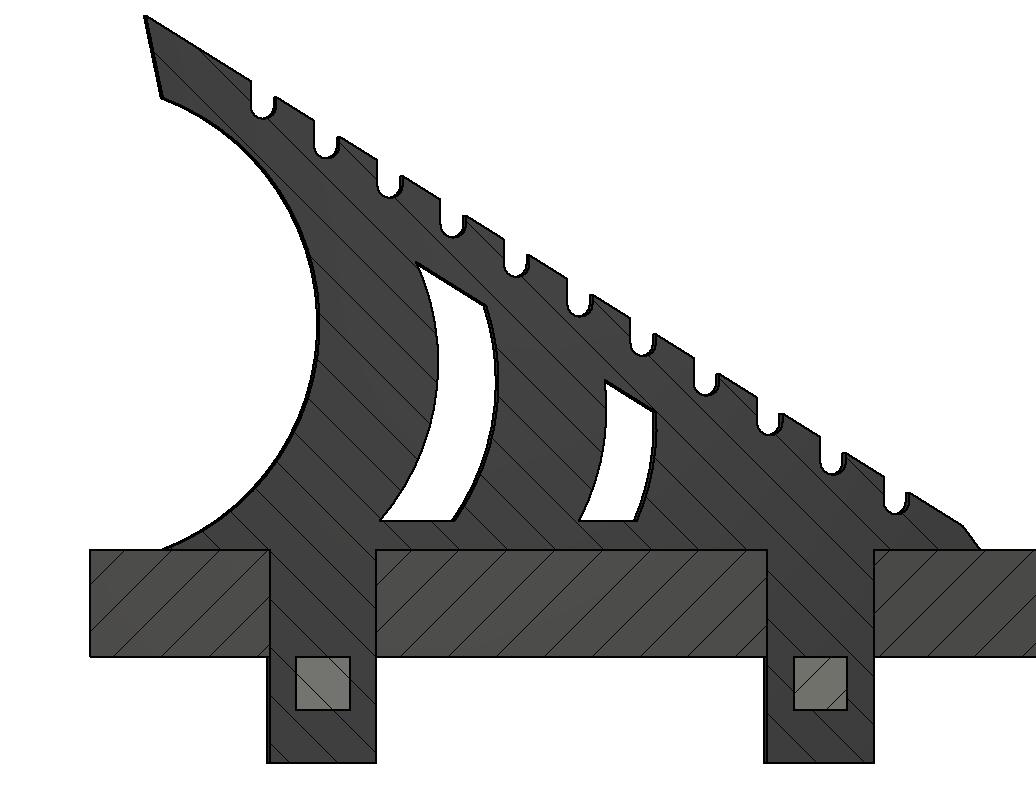
\includegraphics[width=\textwidth]{kassandra/resources/endeMeinerHoffnungInSemi2DStayer.PNG}
    \end{subfigure}%
    \begin{subfigure}{0.5\textwidth}
        \centering
        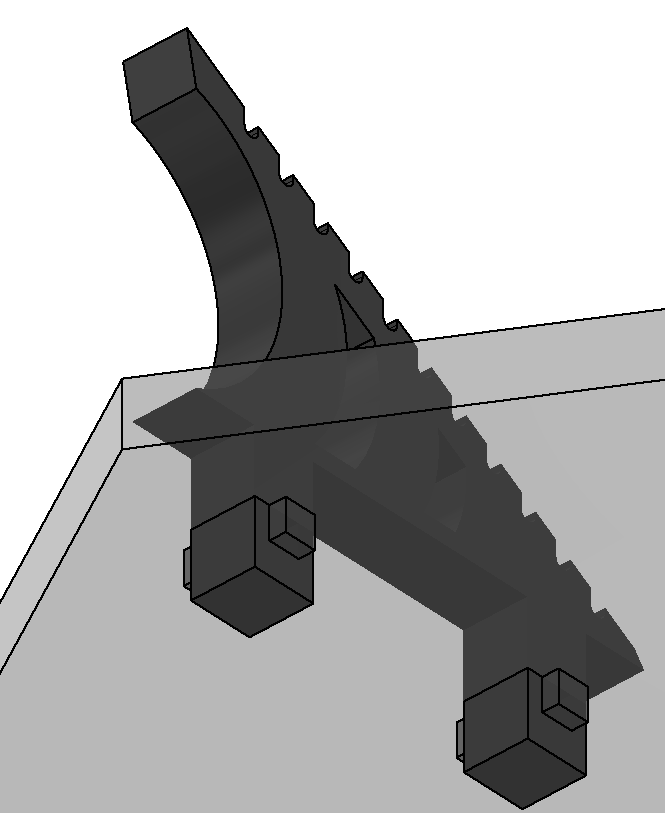
\includegraphics[width=0.7\textwidth]{kassandra/resources/endeMeinerHoffnungIn3DStayer.PNG}
    \end{subfigure}
    \centering
    \caption{Fastening of the supports}
    \label{fig:stayer}
\end{figure}

\subsection{Secondary Coil}

The core of the secondary coil was one of the easier parts to design because it essentially just consists of a 30mm \gls{pmma} tube with a thickness of 3mm. A few millimeters from the top of the tube, a small hole was drilled to guide the wire to the inside and connect it to the top electrode. The 330 turns of 0.35mm wire were then wound by hand and then coated with protective and insulating varnish to prevent the wire from loosening and cross-arcing to occur.

\todo{Das Gerüst für die zwei spulen. Stayer Desgin und funktion.}

\section{Top Electrode}

Technically the tesla coil would also work without a top electrode by simply using the end of the secondary coil's wire as the arcing point. however, given that the wire of the secondary has a small diameter and is made of copper, it would likely melt or at least start to deform when it emits a spark. To ensure the arcing point stays intact, the wire is connected to another material - in this case, a welding electrode made of a tungsten alloy. 

The holder that keeps the electrode at the top of the coil is made of two parts. As seen in figure \ref{fig:top-electrode}, the first is two copper pieces that are kept together with a thread, and in between, the wire of the secondary is clamped. There are also two notches on each to enable fastening and opening with a flat wrench. To mount the tungsten electrode, a press fit was drilled into the top surface of the copper piece. 

The second part is a \gls{pmma} piece with another fit at the top for the copper piece. On one side, there is also a gap to direct the wire of the secondary to the inner part. 

\begin{marginfigure}[-8cm]
    \centering
    \includegraphics[width=0.7\textwidth]{kassandra/resources/endeMeinerHoffnungFürBlitz.PNG}
    \caption{Mounting of the top electrode}
    \label{fig:top-electrode}
\end{marginfigure}

\subsection{It's not a Bug, it's a Feature}

Because the tesla coil driver was very underdesigned, the plasma flame forming on the top electrode was very small and often had to be ignited and stabilized by another conductor held close to it. This was realized by placing a second, ancillary electrode over to the main electrode. This ancillary electrode is held by a canopy-like structure, resting on three \gls{pmma} rods. It was press fitted into a flat copper cylinder, which was loosely screwed into the cap. This way, its height and the gap between the two electrodes could be changed by turning the ancillary electrode. 

\begin{marginfigure}[-3cm]
    \centering
    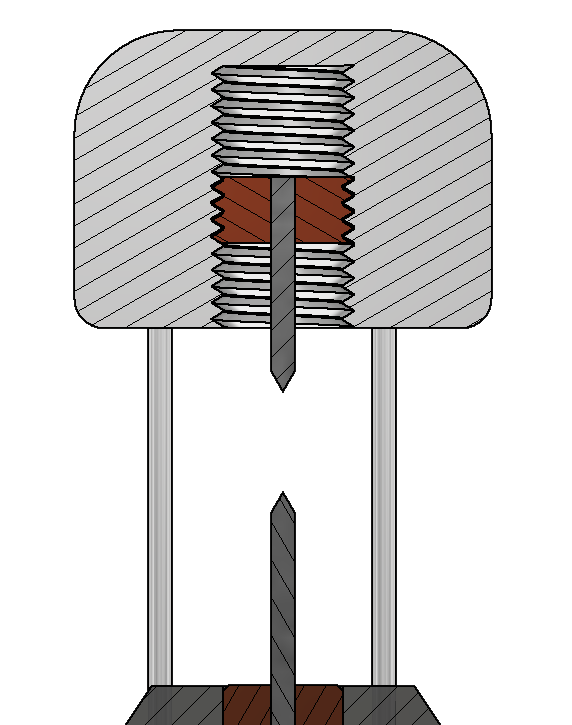
\includegraphics[width=\textwidth]{kassandra/resources/mirGehtsSuperDanke.png}
    \caption{Mounting of the ancillary electrode}
    \label{fig:ancillary-electrode}
\end{marginfigure}

To further examine the effect of the material of the cap, three different versions have been made. One out of \gls{pmma} and two out of Aluminium, one of which is as smooth as possible and one as pointy as possible.

\begin{figure}[h!]
    \centering
    \label{fig:caps}
    \begin{subfigure}[b]{0.4\textwidth}
        \centering
        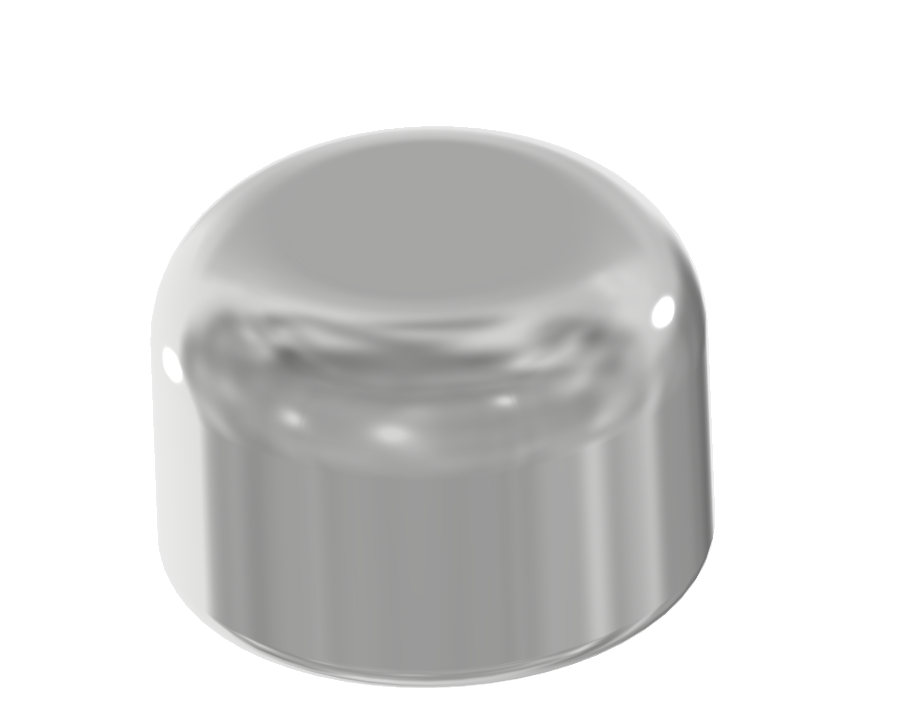
\includegraphics[width=0.9\textwidth]{kassandra/resources/mirGehtsSuperDankeSmooth.png}
    \end{subfigure}
    \hfill
    \begin{subfigure}[b]{0.4\textwidth}
        \centering
        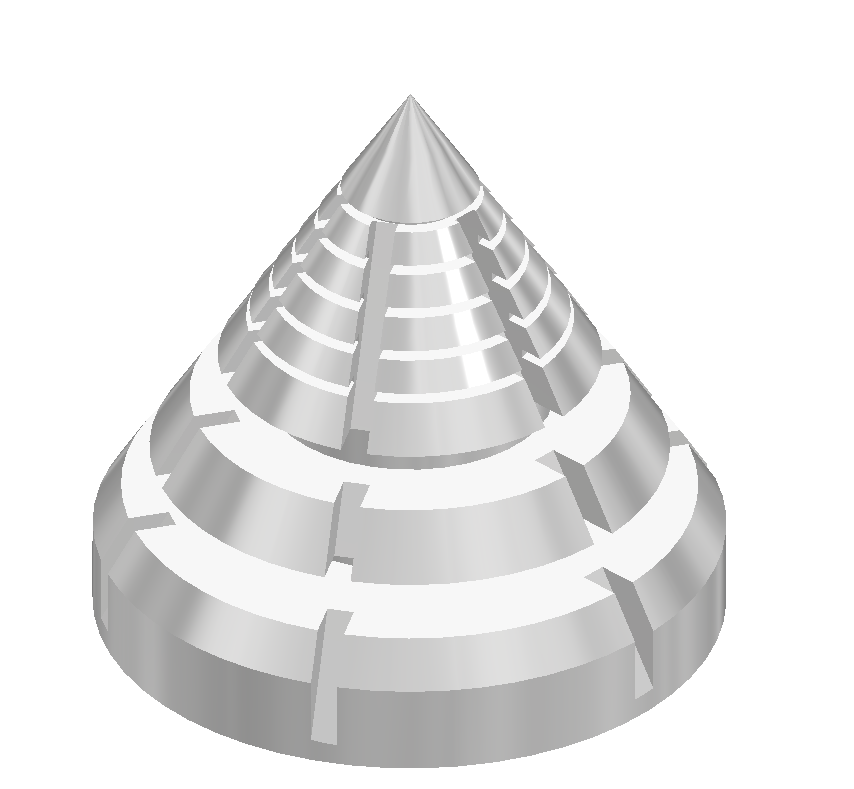
\includegraphics[width=0.9\textwidth]{kassandra/resources/mirGehtsSuperDankeEdgy.png}
    \end{subfigure}
    \caption{Smooth and Pointy Cap}
\end{figure}

While in section \ref{subsec:materials-metals}, it was explained that metals pose a safety hazard, this is not entirely true for the secondary side of the tesla coil. Despite the high voltages of up to several kilovolts present at the top electrode, it is relatively safe to touch. This is because as soon as a low-resistance path to ground, like a human, opens for the current, the voltage drops to a very low level, which means that the resulting current cannot do any harm besides the usual burned skin.

\section{PCB Enclosure}

The general placement of the \gls{pcb}, being right beneath the coils, was already addressed in section \ref{sec:concept-design}. The platform where the secondary coil and the supports for the primary coil are mounted was already designed and chosen to be hexagon-shaped, mainly because it works the best with the six supports. Again, the prototype has the platform resting on top of six pillars to keep everything as modular as possible. The prototype also has only the most essential features and only consists of a framework, this also makes it easier to access the inside of the \gls{pcb} enclosure. The final design would be completely closed off, and the platform would be glued on as with the primary coil’s supports.

\subsection{PCB}

The hexagonal \gls{pcb} was placed in the center of the enclosure right under the secondary, mostly to balance the design. To ensure that the circuit can also give off heat on the bottom side, it cannot be mounted directly onto the enclosure and therefore has to be raised by a few millimeters. This is done by six steps onto which the \gls{pcb} is screwed. 

\subsection{Connections and Things to Press}

To provide the necessary power and the MIDI-Interrupter signal to the PCB as well as the ability to be turned on and off without being plugged out, one side of the PCB enclosure has been dedicated as a control panel. To provide the necessary power, a 5.5 x 2.1 mm barrel plug was used because of its widespread usage. To connect the fiber optic cable, the phototransistor has been mounted directly into the casing, so it is still accessible from the outside. Additionally, a keyswitch\sidenote{This way, only authorized people are able to turn on the tesla coil and feel important} is used to turn on the power, and an ON-OFF-ON switch either routes the output of the phototransistor for interrupted operation, a constant 12V signal for continuous operating, or a 0V signal for no operation to the interrupt input.

\chapter{Printed Circuit Board}

\glspl{pcb} playe an essential role in this project. Breadboards and other prototyping techniques tend to cause issues with parasitic inductances and capacitances and do not work with \gls{smd} components, so \glspl{pcb} were the only way to build up the circuits. Once a \gls{pcb} has been produced, it works reliable and usually does not add any erratic effects. On the downside, however, \glspl{pcb} take a lot of time to design, etch, and solder, and once they are manufactured, they are very inflexible. This means that a new \gls{pcb} had to be made for every prototype..

\section{Component Selection}

Because almost none of the needed components were on hand in the school laboratories, they had to be ordered online. Due to the unique requirements of some parts, like the MOSFET or the \gls{vco}, they were rather hard to find and either very costly or came in an impractical package.

Since all the essential components were only available as \glspl{smd}, most other components were also shifted to \gls{smt} for consistency.


\subsection{ICs}

Most ICs were only available in one package and did not leave much flexibility. The MOSFET driver, \gls{vco}, latch, AND gate, and MOSFET for the phototransistor came in standard SOT and SOIC packages which were easy to solder since they have the pins on their side. The class-E MOSFET and the voltage regulator were somewhat troublesome because their packages had a big metal area on the underside, only indented for one-time reflow soldering. Unfortunately, the class-E MOSFET still needed to be replaced multiple times during the testing process.

\subsection{Passive Elements}

All capacitors and resistors have been ordered in a 0805 package because it is not too big but just big enough to be easy to work with. The small size compared to \glspl{thd} does, however, negatively affect the power rating of resistors and the voltage rating of capacitors, so it had to be made sure that they still operated within the safe operating range. For the capacitors, X7R devices had been chosen, which means that their operating temperature ranges from -55\textdegree C to 125\textdegree C with at most 15\% capacitance change over this range\textsuperscript{\sidecite{epci}}.

%\subsection{Connectors}



% Took some time to find all components

% SMD
% This is the final list of selected components:

\begin{tabular}{@{}lll@{}}
    \toprule
    \textbf{Part name} & \textbf{Footprint} & \textbf{Description}\\\midrule
    BSC12DN20N & PG-TDSON-8 & MOSFET\\
    IX4310 & SOT-23 & MOSFET driver\\
    LTC1799 & SOT-23 & Oscillator\\
    LM7805 & TO252 & Voltage regulator\\
    PKE3316 & Custom THT & boost converter\\
    74HC72 & SOIC127 & D-type latch\\
    TC7SZ08F & SOT-32 & AND gate\\
    RUM001L02 & SOT-723 & MOSFET\\
    47\(\mu\)H choke & Custom SMD &\\
    Various Capacitors & 0805 &\\
    Various Resistors & 0805 &\\
    Potentiometers & PT-10&\\
    Fuse 250mA & 1206 &\\
    Clamp & ? &\\
    Connector & CON06 &\\
    \bottomrule
\end{tabular}

\section{Physical arrangement}
\label{sec:physical-arrangement}

Two things about the placement of the electronics were already certain - that the class-E amplifier and its surroundings were placed in the center of the casing and that the connectors and controls had to be mounted on the side of the casing. The question is how to connect them. Using loose cables would quickly become unclear and cause noise to be picked up by the unamplified interrupter signal from the phototransistor. This could be solved by bundling all signals directly onto a \gls{pcb} and leading them to the main \gls{pcb} via a six pin flat ribbon cable. Additionally, this side board could amplify the interrupter signal to 12V to make it more resilient to induction. 


% Connection to the Coil
% Connection between the PCBs
% Connection to the Perpherals

\section{PCB Layout}

%\section{Manufacturing}
\chapter{Future Improvements}

\section{Battery Pack}